% Main document must include
% \usepackage{tikz}  % for the graphics
% \usepackage{etoolbox}  % for the if-then toggles

\providetoggle{cap-to-dv}
\providetoggle{doe-to-dv}

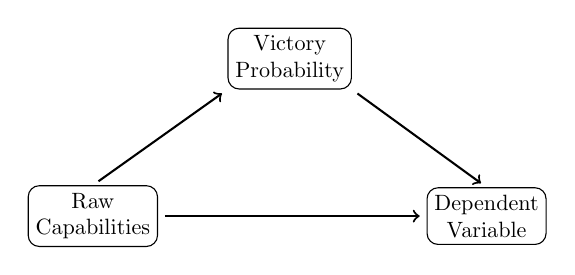
\begin{tikzpicture}[
  var/.style={
    rectangle,
    rounded corners,
    draw=black,
    align=center,
    scale=0.8
    }
  ]
  
  \node[var] (cap) at (0, 0) {Raw\\Capabilities};
  \node[var] (doe) at (2.5, 2) {Victory\\Probability};
  \node[var] (dv) at (5, 0) {Dependent\\Variable};

  \path[->, line width=0.75pt] (cap.north) edge[shorten <=0.25em, shorten >=0.25em] (doe.south west);
  \iftoggle{doe-to-dv}{\path[->, line width=0.75pt] (doe.south east) edge[shorten <=0.25em, shorten >=0.25em] (dv.north);}{}
  \iftoggle{cap-to-dv}{\path[->, line width=0.75pt] (cap.east) edge[shorten <=0.25em, shorten >=0.25em] (dv.west);}{}
\end{tikzpicture}

%%% Local Variables:
%%% mode: latex
%%% TeX-master: "doe"
%%% End:
